\documentclass{standalone}

\usepackage{tikz} % main drawing package used

\usepackage{etoolbox} % for if tests

\usepackage{xcolor} % defining colours
\definecolor{border}{gray}{0.66}
\definecolor{darktan}{rgb}{0.475,0.369,0.263}
\definecolor{tan}{rgb}{0.702,0.541,0.329}
\definecolor{darkred}{rgb}{0.51,0.102,0.059}
\definecolor{red}{rgb}{0.698,0.098,0.027}
\definecolor{darkblue}{rgb}{0.149,0.2,0.0235}
\definecolor{blue}{rgb}{0.18,0.247,0.318}

\newcommand{\thiscirc}{blue} % to store the current colour

\newcommand{\drawblock}[2]{% 
    
    % colour the circles
    \ifnumequal{#1+#2}{2}{\renewcommand{\thiscirc}{tan}}{}
    \ifboolexpr{%
        test {\ifnumequal{#1+#2}{0}}
        or
        test {\ifnumequal{#1+#2}{3}}
    }{\renewcommand{\thiscirc}{red}}{}
    
    % draw them at the right place
    \begin{scope}[shift={(2*#1,2*#2)}]
        \foreach \x/\y in {0/0,0/1,1/0,1/1}{
            \node[circle,draw=dark\thiscirc,fill=\thiscirc,minimum size=5ex] at (\x,\y) {};
        }
    \end{scope}
}

\begin{document}
    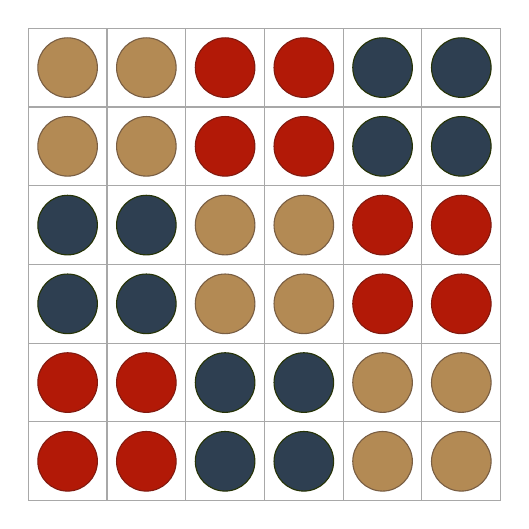
\begin{tikzpicture} % main picture
        
        % draw grid
        \begin{scope}[shift={(-0.5,-0.5)}]
            \foreach \i in {0,...,6}{
                \draw[border] (\i,0) -- (\i,6);
                \draw[border] (0,\i) -- (6,\i);
            }
        \end{scope}
        
        % draw circles
        \foreach \i in {0,1,2}{
            \foreach \j in {0,1,2}{
                \drawblock{\i}{\j}
            }
        }
    \end{tikzpicture}
\end{document}